% vim: tabstop=4 shiftwidth=4 softtabstop=4 expandtab textwidth=80 smarttab

\documentclass{beamer}
\usepackage[cm-default]{fontspec}
\setromanfont{FreeSerif}
\setsansfont{FreeSans}
\setmonofont{FreeMono}
\usepackage{geometry}
\usepackage{tikz}
\usepackage{graphicx}
\graphicspath{ {images/} }
\usetikzlibrary{snakes,arrows,shapes}
\usepackage{amsmath}
%\geometry{screen}
\usepackage{listings}
\lstset{
        language=Ruby,
        morekeywords={bool},
        tabsize=2,
        basicstyle={\ttfamily\tiny},
        numbers=left,
        numberstyle=\tiny,
        stepnumber=1,
        numbersep=4pt,
        showstringspaces=false,
        showspaces=false,
        showtabs=false,
        backgroundcolor=\color{white},
        commentstyle={\em\color{magenta}},
}
\usetheme{Warsaw}
\title[A tale of Multi DC puppet woes]{A tale of migrating to Puppet 3.8 and Multi Datacenter Puppet Infrastructure}
\author{Alexandros Kosiaris <akosiaris@wikimedia.org>}
\institute{GRNOG - 4th Technical Meeting}
\date{02 Dec 2016}
\begin{document}

\AtBeginSubsection[]
{
    \begin{frame}<beamer>
        \frametitle{Layout}
        \tableofcontents[currentsection,currentsubsection]
    \end{frame}
}

\begin{frame}
    \titlepage
\end{frame}

\section{Introduction}

    \begin{frame}{Wikimedia Foundation}
        What is the WMF?
        \begin{itemize}
        \pause \item Non-profit organization focusing on free/open content
        \pause \item No ads, no VC money
        \pause \item Entirely funded by small donors
        \pause \item 280 employees (~60-70 SWE, 20 ops)
        \pause \item Number 5 in Top 10 website companies
        \pause \item 4 Datacenters. 2 main ones, 2 caching, avg latency ~50ms
        \pause \item Server count: \textasciitilde 1200
        \end{itemize}
    \pause Managed via Puppet almost exclusively
    \end{frame}

    \begin{frame}{Puppet in WMF}
        Some numbers:
        \begin{itemize}
            \pause \item 8 git repos containing operations specific code
            \pause \item 50345 lines of Puppet code
            \pause \item 53235 lines of ERB (Embedded Ruby)
            \pause \item 50380 lines of Ruby
        \end{itemize}
        \pause Numbers are not very accurate and do not account for 3rd party code
        imported into repos, include tests/RSpec and comments/whitespace.
    \end{frame}

    \begin{frame}{State pre Q3 2016}
        Agents:
        \begin{itemize}
        \pause \item Run every 30 mins with a randomization in agent run start times
        \pause \item Puppet versions vary from 3.4 to 3.7
        \pause \item Ruby versions vary from 1.8 to 2.1
        \end{itemize}
        \pause Puppetmasters:
        \begin{itemize}
            \pause \item 2 Precise Pangolin (Ubuntu 12.04) boxes
            \pause \item 1 "frontend", 1 "backend"
            \pause \item Puppet versions 3.4
            \pause \item Ruby versions 1.8
        \end{itemize}
    \end{frame}
    \begin{frame}{Puppetmaster CPU usage pre Q3 2016}
        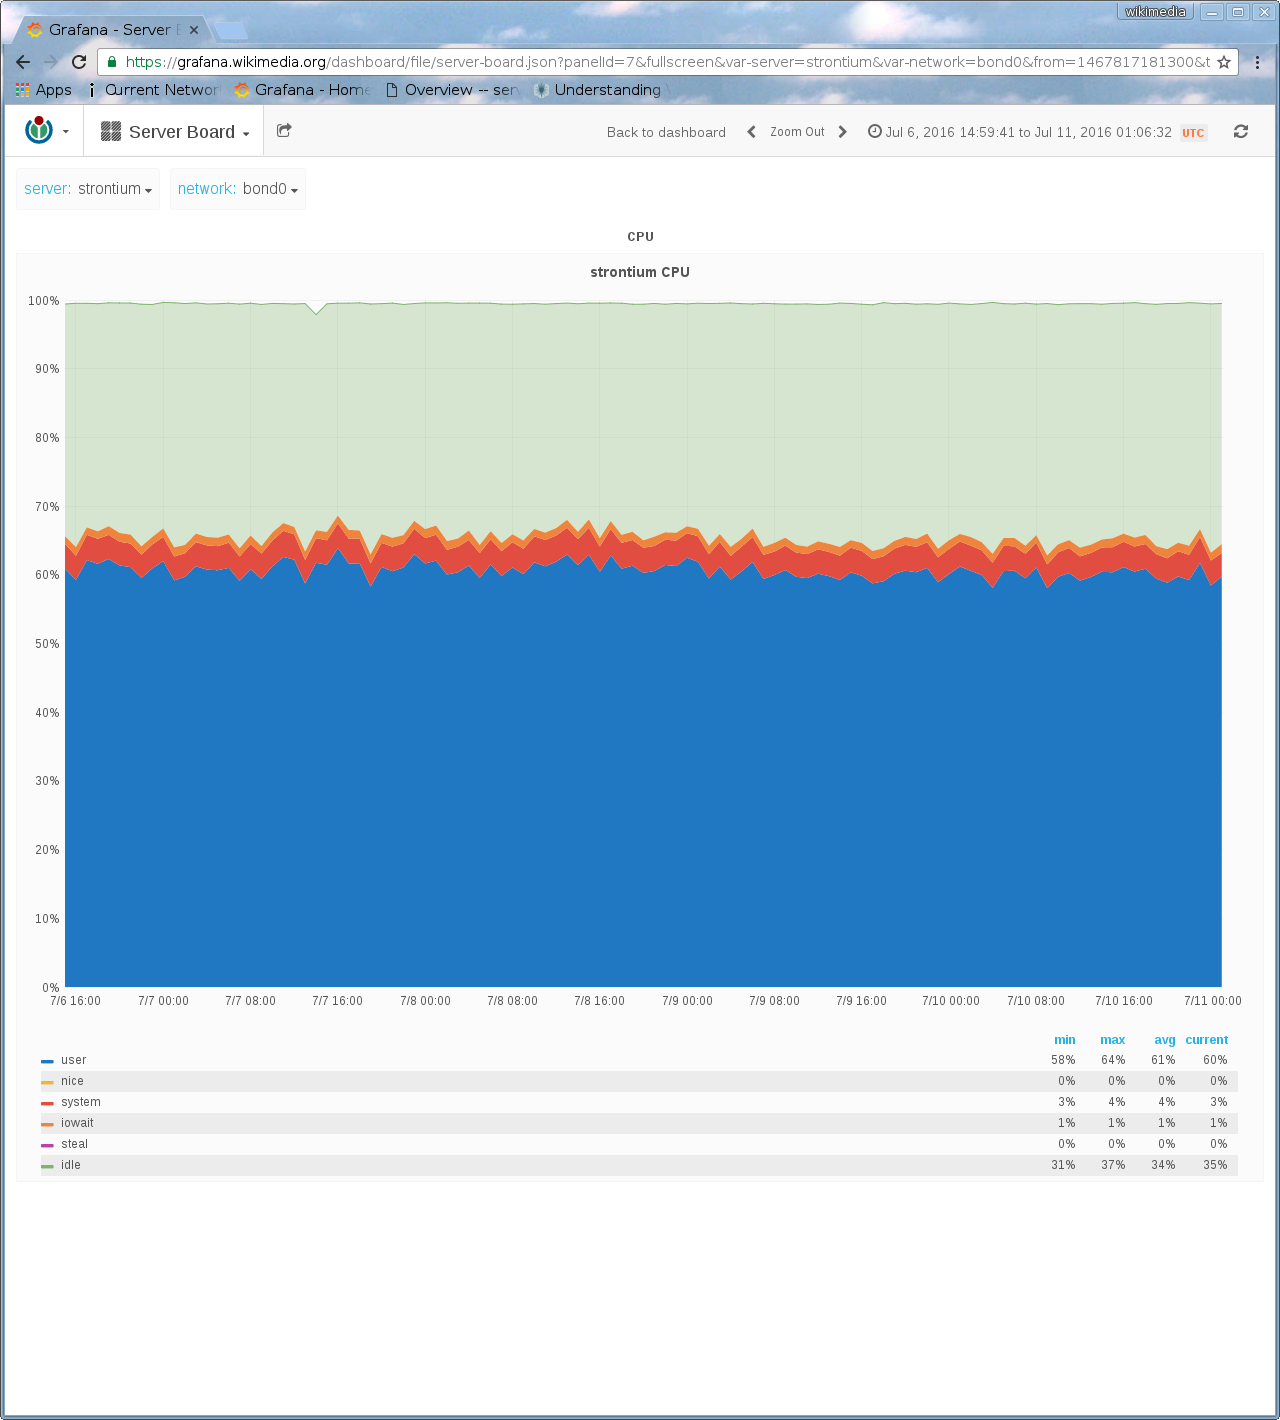
\includegraphics[width=\textwidth, height=\textheight]{cpu_usage_pre_q3_2016.png}
    \end{frame}
    \begin{frame}{State post Q3 2016}
        Agents:
        \begin{itemize}
        \pause \item Run every 30 mins with a randomization in agent run start
            times. Thinking about lowering to 20 though
        \pause \item Puppet versions vary from 3.4 to 3.8 (but with a lower variance)
        \pause \item Ruby versions vary from 1.8 to 2.1 (but with a lower variance)
        \end{itemize}
        Puppetmasters:
        \begin{itemize}
            \pause \item 5 Debian Jessie machines (Debian 8), Ruby version 2.1
            \pause \item 2 "frontends", 3 "backends"
            \pause \item Puppet version 3.8
            \pause \item PuppetDB version 2.3
            \pause \item Ruby version 2.1
        \end{itemize}
    \end{frame}
    \begin{frame}{Puppetmaster CPU usage post Q3 2016}
        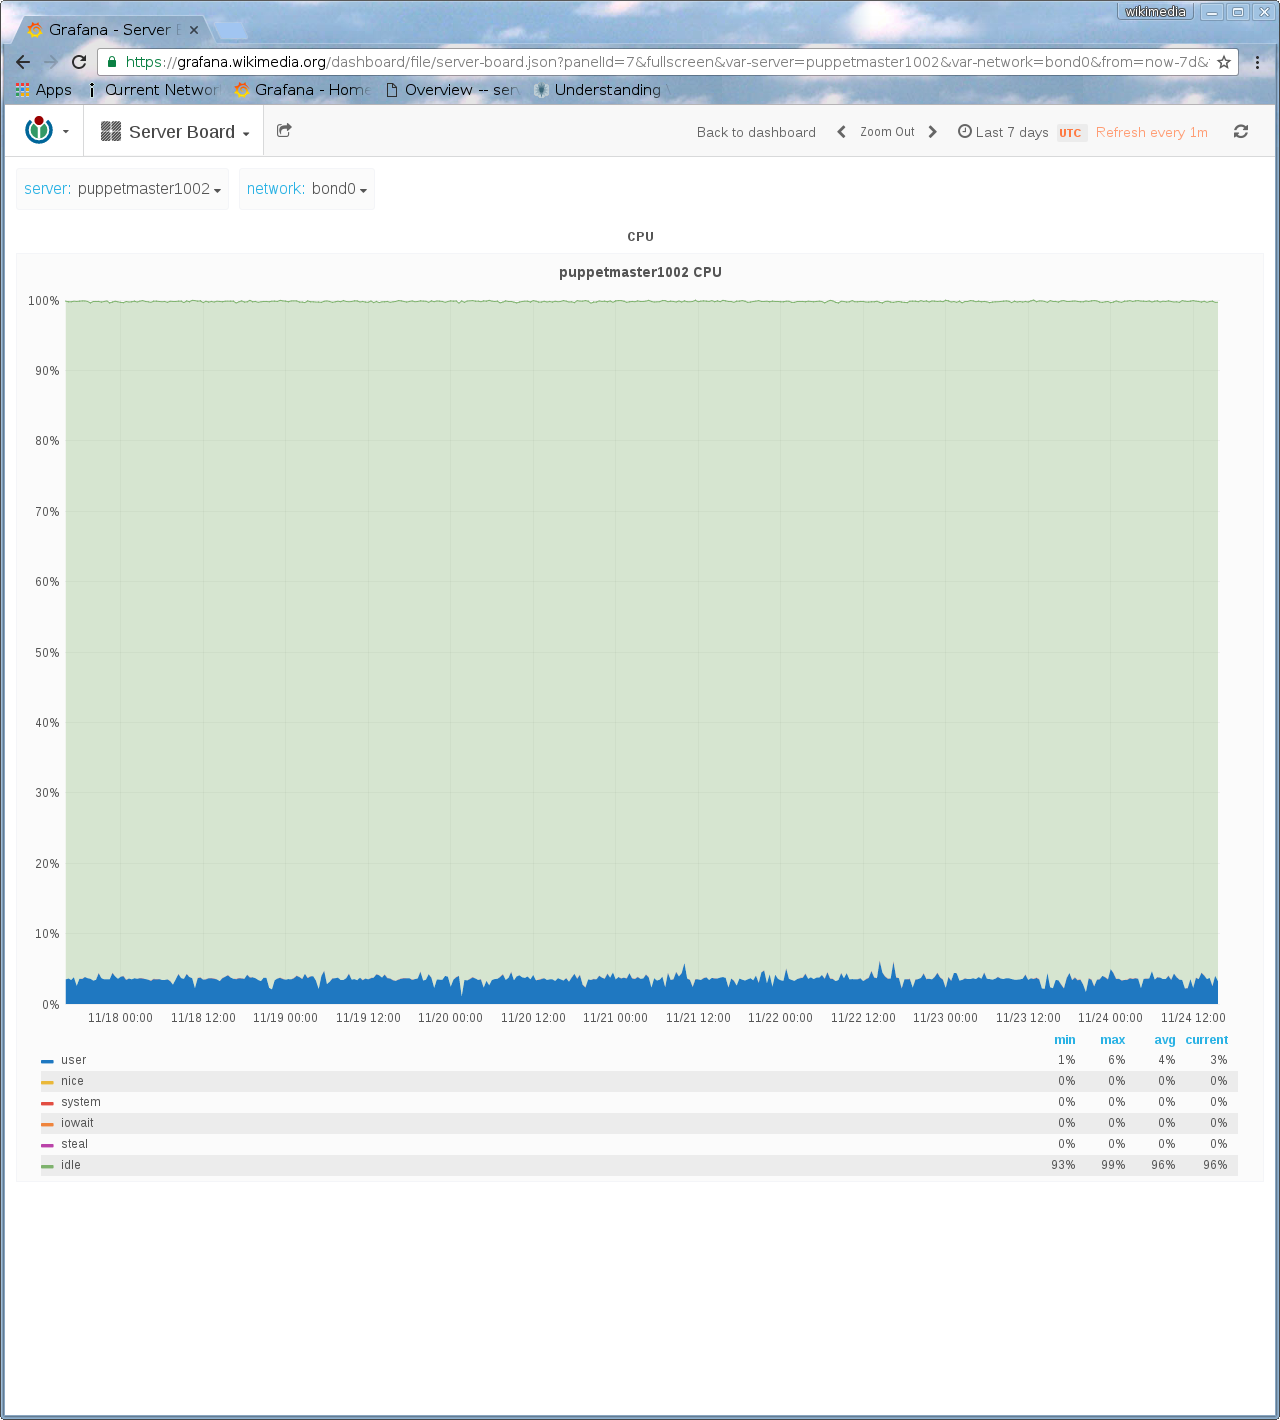
\includegraphics[width=\textwidth, height=\textheight]{cpu_usage_post_q3_2016.png}
    \end{frame}

\section{Architecture}
    \begin{frame}{Terminology}
        \pause Backend:
        \begin{itemize}
            \pause \item An application server using HTTPS as communication protocol
            \pause \item Compiles and serves catalogs and file resources
        \end{itemize}
        \pause Frontend:
        \begin{itemize}
            \pause \item Distributes requests to backends
            \pause \item Also an application server since it serves some resources
        \end{itemize}
        \pause Storedconfigs:
        \begin{itemize}
            \pause \item A database that stores configuration resources
        \end{itemize}
    \end{frame}
    \begin{frame}{Architecture pre Q3 2016}
        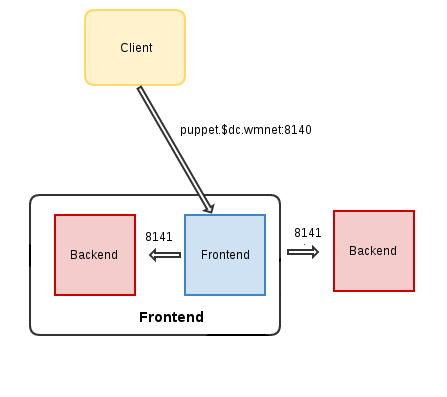
\includegraphics[width=\textwidth, height=\textheight]{Puppet-diagram_pre_q3_2016.png}
    \end{frame}
    \begin{frame}{Architecture pre Q3 2016 (2)}
        Frontend:
        \begin{itemize}
            \pause \item Apache 2.2 with mod\_proxy
            \pause \item Terminates TLS connections and authenticating clients
            \pause \item Reverse Proxy with weighted round-robin to backends (TLS encrypted)
            \pause \item Serves ca, volatile and stores reports, filebuckets exclusively
        \end{itemize}
    \end{frame}
    \begin{frame}{Architecture pre Q3 2016 (3)}
        Backend:
        \begin{itemize}
            \pause \item Apache 2.2 with mod\_passenger
            \pause \item Does the catalog compilations and serves catalogs files
        \end{itemize}
        \pause Storedconfigs:
        \begin{itemize}
            \pause \item A MySQL database, Active Record Ruby Driver communicating with it
        \end{itemize}
    \end{frame}
    \begin{frame}{Architecture post Q3 2016}
        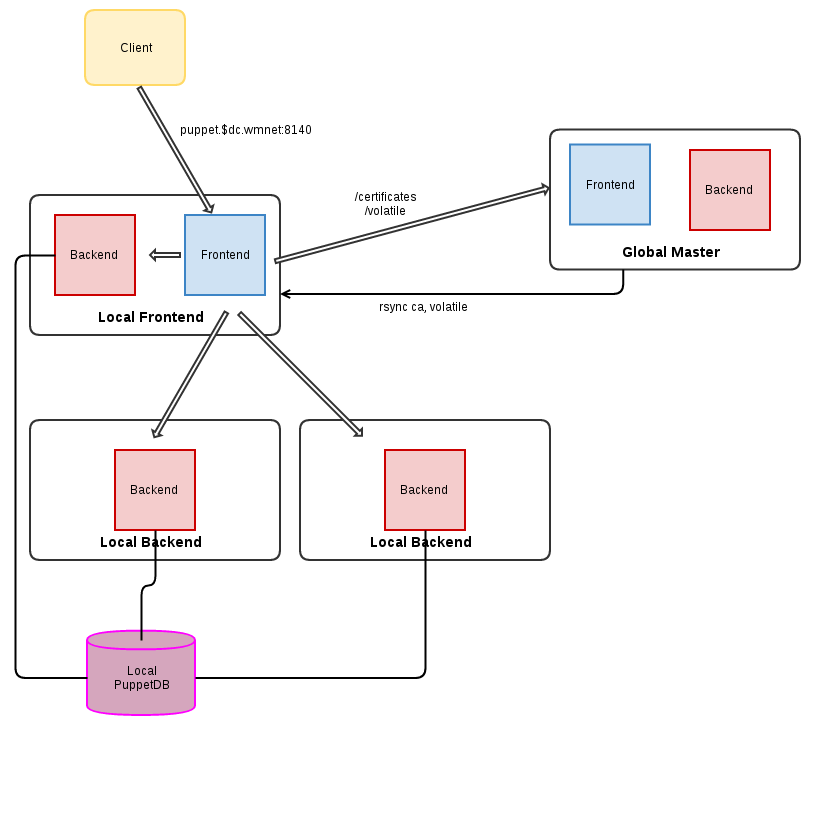
\includegraphics[width=\textwidth, height=\textheight]{Puppet-diagram_post_q3_2016.png}
    \end{frame}
    \begin{frame}{Architecture post Q3 2016 (2)}
        No big changes:
        \begin{itemize}
            \pause \item Apache 2.4 instead of 2.2
            \pause \item Agents now contact closest DC "frontend"
            \pause \item There is now a "Master" frontend for some resources
            \pause \item queries for CA, volatile go to "Master" "frontend"
            \pause \item ca, volatile is being rsynced on frontends (unidirectional )
            \pause \item Backends query puppetDB instead of MySQL for Storedconfigs
        \end{itemize}
    \end{frame}

\section{Migration process}
    \begin{frame}{Getting codebase up to date with puppet 3.8, ruby 2.1}
        \begin{itemize}
            \pause \item Fleet wide catalog compilation on a puppet compiler
            \pause \item Remove all UTF-8 characters
            \pause \item Strings objects handled differently in Ruby 1.9+
            \pause \item Hash mutability is now deprecated and discouraged
            \pause \item Had to repuppetize a few stuff that got erroded over time
        \end{itemize}
    \end{frame}

    \begin{frame}{Get a backend puppetmaster running 3.8}
        \begin{itemize}
            \pause \item New apache Virtualhost on the frontend, new backend only
            \pause \item Switch selectively agents to use the new Virtualhost via \colorbox{lightgray}{server =} directive in puppet.conf
            \pause \item Enable \colorbox{lightgray}{always\_cache\_features = true}, otherwise agent runs take +200\% time
            \pause \item Find out a performance issue that caused catalog bloat by 1500\%
        \end{itemize}
        \pause Marvel at the fact the new backend can serve all the traffic\\
        \pause See the old backend commiting harakiri right after that
    \end{frame}

    \begin{frame}{Get the frontend puppetmaster running 3.8}
        \begin{itemize}
            \pause \item A new frontend running Debian Jessie, puppet 3.8, ruby 2.1
            \pause \item Add a new DNS name
            \pause \item Use once more \colorbox{lightgray}{server =} to selectively switch agents to use it
            \pause \item Handle a few more small issues (e.g. TLS key size)
        \end{itemize}
        \pause Replicate the setup in second DC
    \end{frame}

    \begin{frame}{Start pointing machines to per DC puppetmasters}
        \begin{itemize}
            \pause \item Decide to use DNS SRV records for puppetmaster selection.
            \pause \item Backtrack full speed! 1000+ DNS queries by the agents, 1000\% increase in agent run times in remote DCs
            \pause \item Go with standard DNS A records
        \end{itemize}
        \pause Feel happy!
        \pause Add AAAA records! Feel even happier!
    \end{frame}

    \begin{frame}{Get puppetDB running}
        \begin{itemize}
            \pause \item Setup up master/slave Postgres in Primary/Backup DCs
            \pause \item Compile/Package PuppetDB. Fail, use the vendor packages
            \pause \item nginx for TLS termination proxies to PuppetDBs
            \pause \item Read queries DC local, write queries go to active DC
        \end{itemize}
    \end{frame}

    \begin{frame}{Architecture post Q3 2016 (PuppetDB)}
        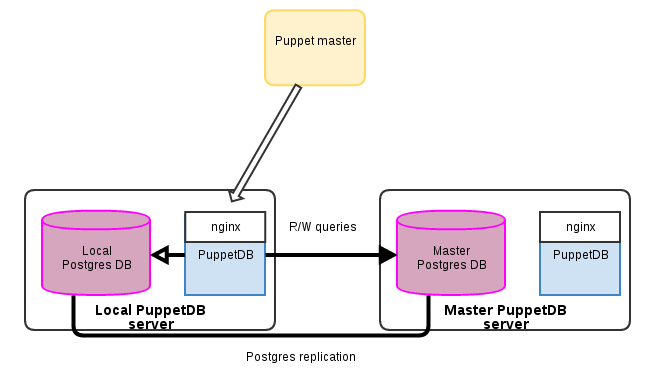
\includegraphics[width=\textwidth, height=\textheight]{Puppetdb-diagram.png}
    \end{frame}

    \begin{frame}{Use/tune puppetDB}
        \begin{itemize}
            \pause \item Remove reports storing
            \pause \item Set Garbage Collection policies
            \pause \item Update scripts to start using it. Ugly ugly syntax
            \pause \item Marvel at the WONTFIX bugs. Still working on them
        \end{itemize}
    \end{frame}
    \begin{frame}{How code gets updated}
        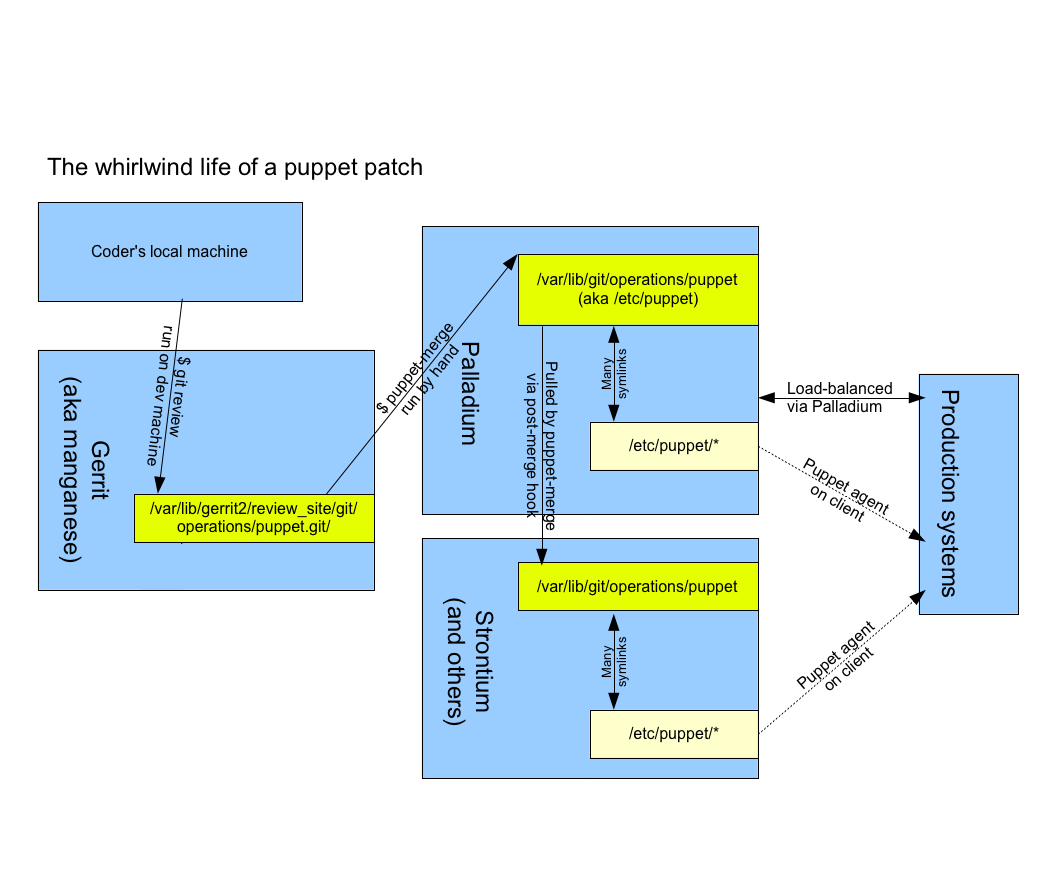
\includegraphics[width=\textwidth, height=\textheight]{Lifeofpuppetpatch.png}
    \end{frame}
    \begin{frame}{Conclusions}
        \begin{itemize}
            \pause \item Multi DC puppetmasters definitely worth it
            \pause \item PuppetDB can be called production ready
            \pause \item Postgres replication is limiting
            \pause \item Read the changelogs many many times over
        \end{itemize}
    \end{frame}
    \begin{frame}{Links}
        \begin{itemize}
            \item https://github.com/akosiaris/presentations
            \item https://github.com/wikimedia/operations-puppet
            \item https://github.com/wikimedia/operations-software-puppet-compiler
        \end{itemize}
    \end{frame}
    \begin{frame}{Questions}
        \begin{center}
            \Huge Questions ?
        \end{center}
    \end{frame}
\end{document}
